\documentclass{beamer}
\usetheme{Madrid}

\usecolortheme{default}
\useinnertheme{circles}
\usepackage[brazilian]{babel}
\usepackage[utf8]{inputenc}
\usepackage{amsmath,mathtools,amsfonts,amssymb}
\usepackage{graphicx}
\usepackage{booktabs}
\usepackage{array}
\usepackage{hyperref}

% Figuras geradas pelo pipeline em confiabilidade/code/resultados/figuras/
\graphicspath{{../../code/resultados/figuras/}}

\title[Confiabilidade (PRONOSTIA)]{Análise de Confiabilidade com Base em Dados Experimentais de Vibração (PRONOSTIA)}
\subtitle{EEE017 --- Confiabilidade de Sistemas}
\author[Felipe / Isabella / Stéphanie]{Felipe Lopes / Isabella Gomes / Stéphanie Barbosa \\ {\footnotesize Prof. Michel Bessani}}
\institute[UFMG]{Universidade Federal de Minas Gerais}
\date{\today}

\begin{document}

% ===================== CAPA =====================
\begin{frame}
    \titlepage
\end{frame}

% ===================== AGENDA =====================
\begin{frame}{Roteiro}
    \tableofcontents
\end{frame}

% =====================================================================
\section{Os Dados}
% =====================================================================

% Slide: a cara dos dados
\begin{frame}{A cara dos dados: vibração bruta}
    \textbf{Fonte:} \textbf{Dataset PRONOSTIA / FEMTO-ST (IEEE PHM 2012)} --- ensaios acelerados em rolamentos até a falha.
    \vspace{0.1cm}
    \begin{itemize}
        \item Cada \texttt{.csv} é um \textit{snapshot}: \textbf{2.560 linhas} de sinal ($=0{,}1$\,s a 25,6\,kHz).
        \item Um \textit{snapshot} novo é salvo a cada \textbf{10\,s}; um rolamento gera \textbf{milhares} deles.
    \end{itemize}
    \vspace{0.1cm}
    \footnotesize
    \begin{tabular}{rrrrcr}
        \toprule
        \textbf{Hour} & \textbf{Min} & \textbf{Sec} & \textbf{$\mu$s} & \textbf{Acc. H ($g$)} & \textbf{Acc. V ($g$)} \\
        \midrule
        10 & 32 & 15 & 123456 & 0,128 & 0,041 \\
        10 & 32 & 15 & 123495 & -0,185 & -0,033 \\
        10 & 32 & 15 & 123534 & 0,009 & 0,112 \\
        \bottomrule
    \end{tabular}
    \normalsize
    \vspace{0.15cm}
    \begin{block}{Lendo as colunas}
        \footnotesize \textbf{Hour/Min/Sec/$\mu$s}: carimbo de tempo da amostra ($\mu$s $=$ microssegundos). \textbf{Acc. H / Acc. V}: aceleração \textbf{horizontal} e \textbf{vertical} em $g$. O ensaio é \textbf{interrompido} quando a vibração ultrapassa \textbf{20\,g} (falha funcional: evita dano catastrófico à bancada).
    \end{block}
\end{frame}

% Slide: a bancada
\begin{frame}{O Dataset PRONOSTIA (FEMTO-ST)}
    \begin{columns}
        \column{0.5\textwidth}
        \footnotesize
        \textbf{O que é medido:} não há motor/bomba --- a bancada testa o \textbf{próprio rolamento} até quebrar. Um motoredutor gira o eixo e um macaco pneumático aplica carga radial sobre o rolamento-alvo.
        \vspace{0.15cm}

        \textbf{Operação (run-to-failure):}
        \begin{itemize}
            \item Carga radial extrema: até \textbf{5.000\,N} ($\approx$\,510\,kgf, $\sim$meia tonelada).
            \item Rotação constante (1500--1800\,RPM, fixada pela bancada).
        \end{itemize}
        \column{0.5\textwidth}
        \begin{block}{Por que ``acelerado''?}
            \footnotesize A carga colossal força a \textbf{fadiga natural} (trincas, descascamento) em \textbf{1--7\,h}, em vez de defeitos usinados. Obtém-se a \textbf{vida real} de cada unidade.
        \end{block}
        \footnotesize \textit{PRONOSTIA} é o nome da plataforma experimental do instituto FEMTO-ST (não há sigla oficial por extenso).
    \end{columns}
\end{frame}

% Slide: os modos de falha / condicoes
\begin{frame}{O conjunto de dados estudado: 17 rolamentos}
    \footnotesize
    São \textbf{17 rolamentos} divididos em \textbf{3 condições de operação} (carga + rotação). A unidade é identificada pela pasta \texttt{Bearing\{condição\}\_\{unidade\}}:
    \vspace{0.1cm}

    \begin{tabular}{clcc}
        \toprule
        \textbf{Condição} & \textbf{Carga / Rotação} & \textbf{Unidades} & \textbf{Qtd.} \\
        \midrule
        1 & 4000\,N / 1800\,RPM & \texttt{Bearing1\_1 .. 1\_7} & 7 \\
        2 & 4200\,N / 1650\,RPM & \texttt{Bearing2\_1 .. 2\_7} & 7 \\
        3 & 5000\,N / 1500\,RPM & \texttt{Bearing3\_1 .. 3\_3} & 3 \\
        \midrule
        \multicolumn{3}{r}{\textbf{Total}} & \textbf{17} \\
        \bottomrule
    \end{tabular}
    \normalsize
    \vspace{0.15cm}
    \begin{itemize}
        \item \textbf{Todo} o dataset é usado: os 17 são agrupados como \textbf{uma única população} de ``rolamento sob carga acelerada''.
        \item Diferenciação entre unidades $=$ pelo nome da pasta (não há ``polos''; a rotação é imposta diretamente pela bancada).
    \end{itemize}
    \vspace{0.1cm}
    \begin{block}{Por que só a aceleração horizontal?}
        \footnotesize Há \textbf{2 acelerômetros} (horizontal e vertical). A carga é aplicada na \textbf{vertical}, deixando a estrutura mais rígida nesse eixo; o \textbf{horizontal} é mais sensível ao defeito em formação e exibe a tendência de degradação mais clara --- é a escolha padrão na literatura do PRONOSTIA.
    \end{block}
\end{frame}

% Slide: frequencia de amostragem
\begin{frame}{Frequência de amostragem e duração}
    \begin{columns}
        \column{0.55\textwidth}
        \begin{itemize}
            \item Taxa de amostragem: \textbf{25,6\,kHz} (25.600 amostras/s).
            \item Cada arquivo (\textit{snapshot}): \textbf{2.560 linhas} (duração de 0,1\,s).
            \item Medições (novos arquivos) salvas a cada 10 segundos.
        \end{itemize}
        \column{0.45\textwidth}
        \begin{alertblock}{Desafio dos Dados}
            Para a vida inteira de um rolamento (que dura algumas horas), temos milhares de arquivos \texttt{.csv}.\\[4pt]
            Precisamos extrair uma única \textit{feature} contínua que resuma toda a degradação!
        \end{alertblock}
    \end{columns}
\end{frame}

% =====================================================================
\section{Estrutura dos Dados}
% =====================================================================

% Slide: estrutura de pastas
\begin{frame}[fragile]{Estrutura de pastas: \textit{Learning} vs \textit{Full Test}}
    \footnotesize
    \begin{tabular}{ll}
        \toprule
        \textbf{Pasta / Set} & \textbf{Conteúdo} \\
        \midrule
        \texttt{Learning\_set} & 6 rolamentos (Ex: \texttt{Bearing1\_1}) \\
        \texttt{Full\_Test\_Set} & 11 rolamentos (Ex: \texttt{Bearing1\_3}) \\
        \bottomrule
    \end{tabular}
    \normalsize
    \vspace{0.15cm}
    \begin{block}{De onde vem essa divisão (desafio IEEE PHM 2012)}
        \footnotesize
        \begin{itemize}\setlength{\itemsep}{2pt}
            \item \textbf{\texttt{Learning\_set} (treino):} trajetórias \textbf{completas} (do rolamento são até a falha), entregues aos participantes para \textbf{treinar} modelos de prognóstico.
            \item \textbf{\texttt{Full\_Test\_Set} (teste):} no desafio, esses dados vinham \textbf{truncados} (cortados antes da falha) e o objetivo era \textbf{prever a vida restante (RUL)}. Esta versão ``\textit{Full}'' traz a vida \textbf{completa} até a falha.
        \end{itemize}
    \end{block}
    \vspace{0.05cm}
    \begin{itemize}\setlength{\itemsep}{1pt}
        \item Para confiabilidade precisamos da \textbf{vida inteira} de cada unidade $\Rightarrow$ usamos os dois conjuntos, \textbf{pondo os 17 juntos} como uma só população.
        \item Cada rolamento contém milhares de arquivos \texttt{acc\_xxxxx.csv}.
    \end{itemize}
\end{frame}

% Slide: tabela original vs gerada
\begin{frame}{De milhares de amostras a uma feature}
    \footnotesize
    \textbf{Entrada:} $\sim$43.000 arquivos \texttt{.csv} no total. Cada um com \textbf{2.560 linhas}.
    \vspace{0.1cm}

    \begin{block}{O indicador de degradação: RMS de banda}
        O sinal de cada \textit{snapshot} vira um \textbf{indicador de degradação} $=$ o valor \textbf{RMS} (Raiz Quadrada Média) da vibração, que mede a \textbf{energia vibratória}. Conforme o rolamento se degrada, trincas e descascamentos aumentam os choques mecânicos, elevando o RMS monotonicamente.\\[3pt]
        \textbf{Banda usada: 10\,Hz--10\,kHz} (banda ampla, via espectro de Welch). Como a fadiga gera energia em \textbf{todo o espectro} (impactos de banda larga), integrar quase toda a faixa captura melhor a severidade do que uma banda estreita.\\[3pt]
        Assim, condensamos as 2.560 linhas de um instante em \textbf{um único número}.
    \end{block}
    \vspace{0.1cm}
    \textbf{Saída (\texttt{features.csv}):} a história de vida de cada rolamento.
    \vspace{0.05cm}

    \begin{tabular}{llrr}
        \toprule
        \textbf{rolamento} & \textbf{snapshot} & \textbf{tempo (h)} & \textbf{valor (RMS)} \\
        \midrule
        Bearing1\_1 & acc\_00001.csv & 0,000 & 0,431 \\
        Bearing1\_1 & acc\_00002.csv & 0,002 & 0,428 \\
        $\cdots$ & $\cdots$ & $\cdots$ & $\cdots$ \\
        Bearing1\_1 & acc\_02803.csv & 7,783 & 20,01 \\
        \bottomrule
    \end{tabular}
    \normalsize
\end{frame}

% =====================================================================
\section{Metodologia}
% =====================================================================

% Slide: features = trajetoria de degradacao no tempo real
\begin{frame}{Passo 1--2: As \textit{features} traçam a degradação no tempo}
    \begin{columns}
        \column{0.52\textwidth}
        \footnotesize
        \textbf{Glossário (eixos da curva):}
        \begin{itemize}
            \item \textbf{\textit{Baseline}}: vibração do rolamento \textbf{saudável} (início do teste).
            \item \textbf{Fase de defeito}: a vibração sobe à medida que a trinca cresce.
            \item \textbf{Falha funcional}: vibração atinge \textbf{20\,g} $\Rightarrow$ bancada para.
        \end{itemize}
        \begin{alertblock}{Aqui as \textit{features} VIRAM tempo}
            \footnotesize Cada \textit{snapshot} tem um \textbf{carimbo de tempo real}. Plotar RMS $\times$ tempo dá a \textbf{trajetória de degradação verdadeira} --- o tempo de falha é \textbf{lido direto}, não simulado (diferente de datasets de \textit{snapshots} sem eixo de vida).
        \end{alertblock}
        \column{0.48\textwidth}
        \begin{center}
            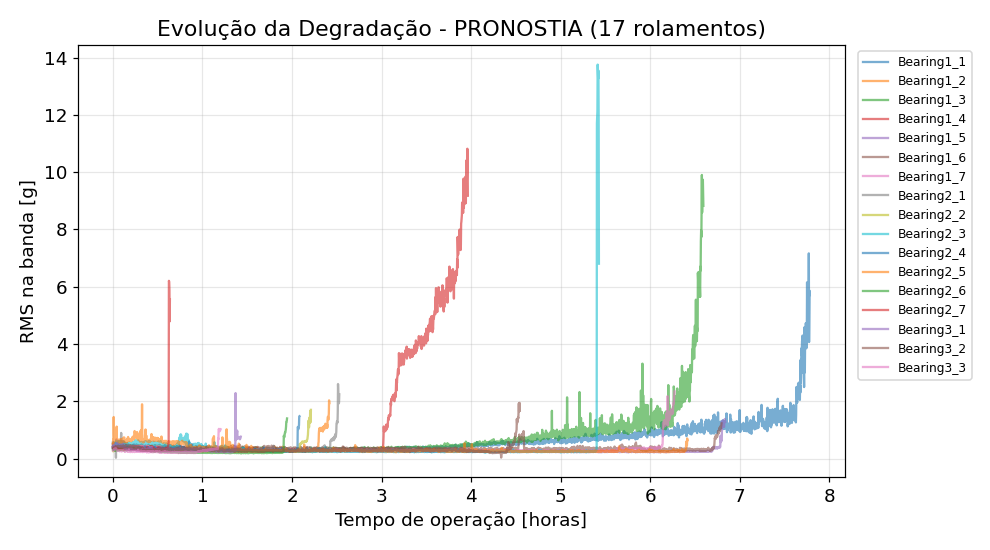
\includegraphics[width=\linewidth]{p1_assinatura_pronostia_all.png}
        \end{center}
        \scriptsize Cada curva $=$ um rolamento. O RMS sobe e dispara no fim da vida.
    \end{columns}
\end{frame}

% Slide: geracao dos TTF (agora reais)
\begin{frame}{Passo 2: Extração dos Tempos Até a Falha (TTF)}
    \begin{columns}
        \column{0.40\textwidth}
        \scriptsize
        Diferente de datasets de \textit{snapshots}, \textbf{não simulamos} tempos de falha: os ensaios são \textbf{run-to-failure}. O TTF de cada rolamento é o \textbf{tempo do último arquivo} antes do desligamento (vibração $>20$\,g).
        \vspace{0.15cm}

        \begin{block}{Sem censura}
            \scriptsize Os 17 rolamentos foram testados até quebrar $\Rightarrow$ \textbf{nenhuma censura} (\textit{censura}$=0$ para todos). Temos a vida \textbf{exata} de todo o lote.
        \end{block}
        \column{0.60\textwidth}
        \scriptsize
        \textbf{Tabela gerada (\texttt{ttf.csv}) --- 17 vidas:}
        \vspace{0.05cm}

        \tiny
        \begin{tabular}{lcr@{\hskip 8pt}lcr}
            \toprule
            \textbf{Rol.} & \textbf{Carga (N)} & \textbf{TTF (h)} & \textbf{Rol.} & \textbf{Carga (N)} & \textbf{TTF (h)} \\
            \midrule
            1\_1 & 4000 & 7,78 & 2\_3 & 4200 & 6,42 \\
            1\_2 & 4000 & 2,42 & 2\_4 & 4200 & 1,94 \\
            1\_3 & 4000 & 6,27 & 2\_5 & 4200 & 0,64 \\
            1\_4 & 4000 & 2,53 & 2\_6 & 4200 & 1,43 \\
            1\_5 & 4000 & 2,21 & 2\_7 & 4200 & 4,54 \\
            1\_6 & 4000 & 5,43 & 3\_1 & 5000 & 6,84 \\
            1\_7 & 4000 & 2,08 & 3\_2 & 5000 & 6,80 \\
            2\_1 & 4200 & 6,59 & 3\_3 & 5000 & 1,20 \\
            2\_2 & 4200 & 3,96 & & & \\
            \bottomrule
        \end{tabular}
    \end{columns}
\end{frame}

% Slide: ajuste de distribuicoes (parte 1 - parametros)
\begin{frame}{Passo 3: ajuste de distribuições de vida}
    \footnotesize
    Sobre as 17 vidas (TTF), ajusta-se por \textbf{máxima verossimilhança}:
    \begin{itemize}\setlength{\itemsep}{1pt}
        \item Exponencial ($\lambda$);\quad Weibull ($\beta$, $\eta$);\quad Lognormal ($\mu$, $\sigma$).
    \end{itemize}
    \vspace{0.1cm}
    \footnotesize
    \begin{tabular}{cll}
        \toprule
        \textbf{Par.} & \textbf{Significado} & \textbf{Distribuição} \\
        \midrule
        $\lambda$ & taxa de falha (constante) & Exponencial \\
        $\beta$ & forma (inclinação da falha) & Weibull \\
        $\eta$ & escala / vida característica (h) & Weibull \\
        $\mu$ & média do $\ln(t)$ & Lognormal \\
        $\sigma$ & desvio-padrão do $\ln(t)$ & Lognormal \\
        \bottomrule
    \end{tabular}
    \normalsize
    \vspace{0.1cm}
    \begin{block}{O que é verossimilhança e como entra aqui (MLE)}
        \scriptsize \textbf{Verossimilhança} $=$ a probabilidade de os dados observados terem sido gerados por uma dada distribuição, vista como \textbf{função dos parâmetros}: $L(\theta)=\prod_{i=1}^{17} f(t_i;\theta)$ (produto das densidades nas 17 vidas). O \textbf{MLE} escolhe o $\theta$ ($\beta,\eta,\dots$) que \textbf{maximiza} $L$ --- ou seja, a distribuição sob a qual os 17 TTFs medidos são os \textbf{mais plausíveis}. Os parâmetros saem direto dessas 17 vidas, sem ajuste manual.
    \end{block}
\end{frame}

% Slide: ajuste de distribuicoes (parte 2 - selecao por AICc)
\begin{frame}{Passo 3: seleção do modelo (AICc)}
    \begin{columns}
        \column{0.5\textwidth}
        \begin{block}{O que é o AICc}
            \footnotesize \textbf{AICc} (\textit{Akaike Information Criterion corrected}): mede o ajuste \textbf{penalizando} o nº de parâmetros $k$ (evita premiar a distribuição mais complexa). \textbf{Menor vence.}\\[3pt]
            $\text{AICc} = 2k - 2\ln(\hat{L}) + \dfrac{2k(k+1)}{n-k-1}$\\[3pt]
            {\tiny *Akaike (1974), correção de Sugiura (1978) para amostra pequena.}
        \end{block}
        \column{0.5\textwidth}
        \begin{center}
            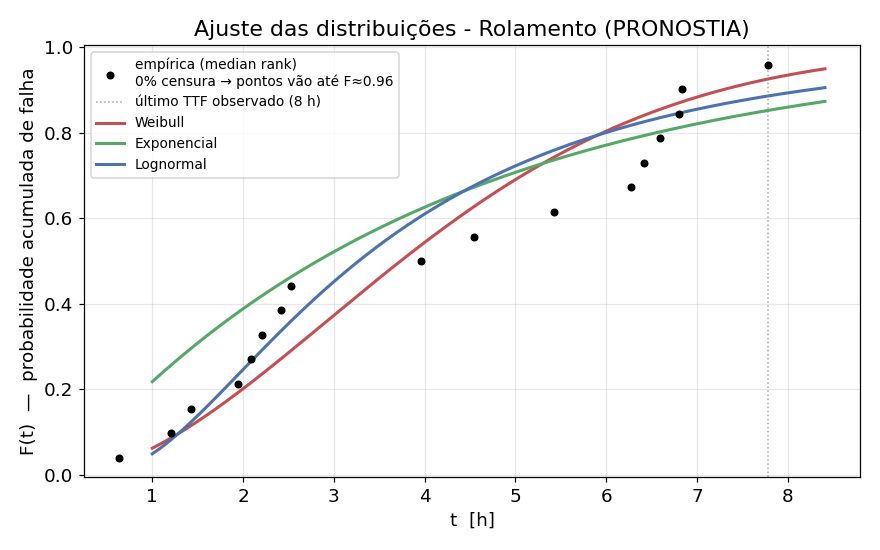
\includegraphics[width=\linewidth]{p3_cdf_pronostia_all.png}
        \end{center}
        \scriptsize \textbf{CDF} $F(t)$: probabilidade de já ter falhado até $t$ (pontos $=$ os 17 dados; curvas $=$ modelos). \textbf{\textit{Median ranks} (Benard)}: posição estimada de cada falha na CDF, $\frac{i-0{,}3}{n+0{,}4}$, para plotar os dados sem viés.
    \end{columns}
\end{frame}

% Slide: tabela parametros e vencedora
\begin{frame}{Passo 3: parâmetros e distribuição vencedora}
    \scriptsize
    \begin{tabular}{lcccc}
        \toprule
        \textbf{Modo} & \textbf{Melhor} & $\beta$ & $\eta$ (h) & \textbf{AICc (W / E / L)} \\
        \midrule
        Rolamento (PRONOSTIA) & \textbf{Weibull} & 1,80 & 4,51 & \textbf{80} / 84 / 82 \\
        \bottomrule
    \end{tabular}
    \vspace{0.3cm}
    \begin{block}{A supremacia da Weibull}
        \scriptsize A distribuição \textbf{Weibull} venceu no critério estatístico (menor AICc). Além disso, ela é fundamental na engenharia por oferecer interpretação física direta do parâmetro de forma $\beta$ na curva da banheira. O $\eta$ é a \textbf{vida característica}: por definição da Weibull, $R(\eta)=e^{-(\eta/\eta)^\beta}=e^{-1}$, então em $t=\eta$ já falharam $1-e^{-1}\approx 63\%$ das unidades. É \textbf{propriedade matemática} (vale para qualquer $\beta$), não convenção de engenharia.
    \end{block}
\end{frame}

% Slide: bootstrap
\begin{frame}{Passo 4: intervalos de confiança por \textit{bootstrap}}
    \begin{columns}
        \column{0.5\textwidth}
        \scriptsize
        \textbf{Como é calculado} --- repete-se o procedimento abaixo $r=10^4$ vezes ($r$ $=$ número de \textbf{reamostragens}):
        \begin{enumerate}\setlength{\itemsep}{0pt}
            \item sorteia, \textbf{com reposição}, 17 TTF da amostra original;
            \item reajusta a Weibull $\rightarrow$ par $(\beta_b,\eta_b)$.
        \end{enumerate}
        IC 95\% $=$ [percentil 2,5\% ; 97,5\%] das $r=10^4$ estimativas:
        $$\text{IC}_{\beta}=\big[\,\beta_{(2{,}5\%)},\ \beta_{(97{,}5\%)}\big].$$
        \begin{block}{O que são $\beta$, $\eta$ e $R(t)$}
            \tiny
            $\beta$ \textbf{(forma)}: inclinação da falha --- localiza na banheira ($\beta{>}1$ desgaste).\\
            $\eta$ \textbf{(escala)}: ``vida característica'', tempo em que $\approx 63\%$ falham.\\
            $R(t)$ \textbf{(confiabilidade)}: prob.\ de \textbf{sobreviver} além de $t$: $R(t)=e^{-(t/\eta)^{\beta}}$.
        \end{block}
        \column{0.5\textwidth}
        \begin{center}
            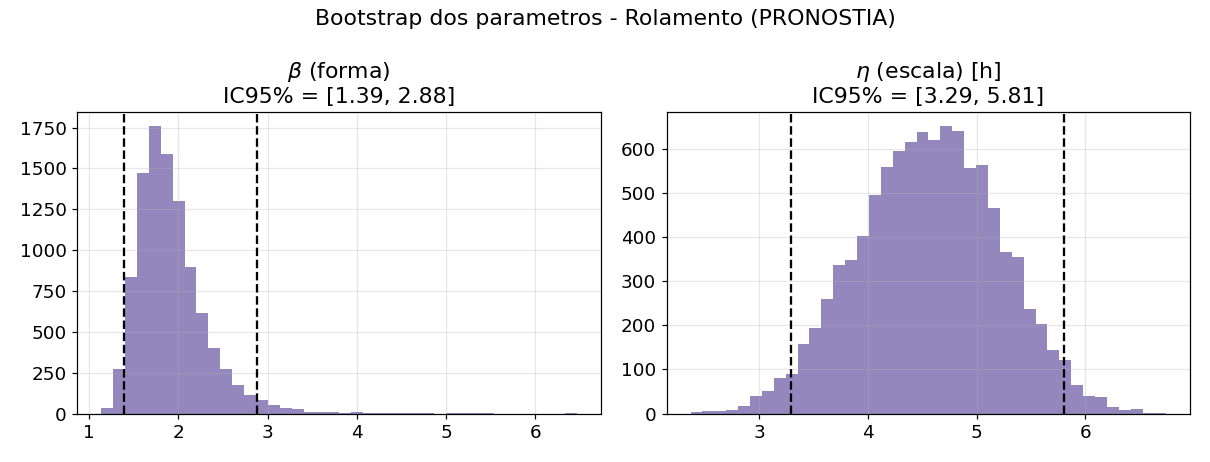
\includegraphics[width=\linewidth]{p4_bootstrap_pronostia_all.png}
        \end{center}
        {\tiny\linespread{0.82}\selectfont Histogramas das $10^4$ reamostras: \textbf{eixo $x$} $=$ valor do parâmetro ($\beta$ ou $\eta$), \textbf{eixo $y$} $=$ frequência. As \textbf{linhas verticais tracejadas} marcam os limites do \textbf{IC 95\%}. É a distribuição \textbf{amostral} da estimativa (sino pelo TLC); essa forma não tem relação com o $\beta$ da vida do rolamento.\par}
        \vspace{0.1cm}
        \begin{center}
            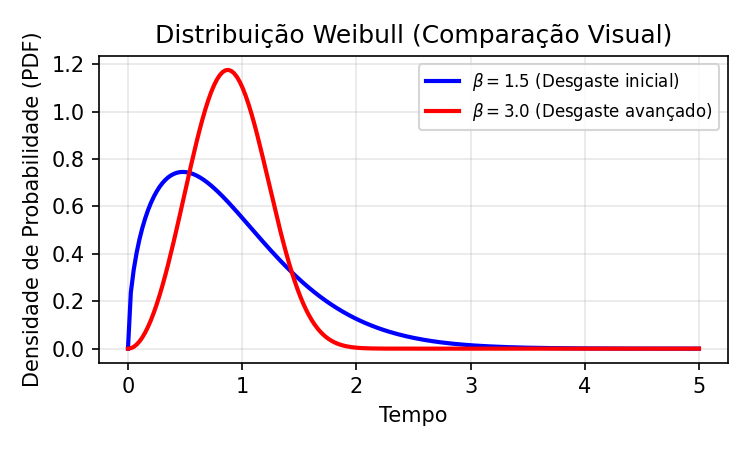
\includegraphics[width=0.62\linewidth]{weibull_generica.png}
        \end{center}
        {\tiny Efeito de $\beta$ na forma da curva (exemplo: $\beta{=}1{,}5$ vs $\beta{=}3{,}0$).}
    \end{columns}
\end{frame}

% =====================================================================
\section{Índices de Confiabilidade}
% =====================================================================

% Slide: indices finais
\begin{frame}{Passo 5: índices finais de confiabilidade}
    \footnotesize
    \begin{tabular}{lrcl}
        \toprule
        \textbf{Modo} & \textbf{MTTF (h)} & \textbf{Disponibilidade} & \textbf{Estágio ($\beta$)} \\
        \midrule
        Rolamento (PRONOSTIA) & 4,0 & 0,1449 & desgaste ($\beta{=}1{,}80$) \\
        \bottomrule
    \end{tabular}
    \scriptsize
    \vspace{0.2cm}
    \begin{itemize}
        \item \textit{MTTF} (Mean Time To Failure) $=$ valor esperado da Weibull;\\ \textit{MTTR} (Mean Time To Repair) $=24$\,h;\\ \textit{A} (Disponibilidade) $= \dfrac{\textit{MTTF}}{\textit{MTTF}+\textit{MTTR}}$.
        \item O parâmetro $\beta=1{,}80$ confirma que a falha é guiada por \textbf{desgaste e fadiga} (taxa de falha crescente).
        \item O MTTF é muito baixo (4 horas) e a disponibilidade pequena (14\%) porque a máquina foi submetida a uma carga radial colossal para forçar a quebra rapidamente, típico de um \textbf{Ensaio Acelerado de Vida} (ALT).
    \end{itemize}
    \vspace{0.05cm}
    \begin{block}{De onde vem o MTTR $=24$\,h}
        \tiny É um \textbf{valor de engenharia assumido} (definido em \texttt{config.py}), não medido: representa o tempo típico para \textbf{substituir um rolamento} ($\sim$1--2 turnos de trabalho). Como o MTTF acelerado é só $\sim$4\,h, esse reparo de 1 dia derruba a disponibilidade --- artefato do ensaio acelerado, não de uso real.
    \end{block}
\end{frame}

% Slide: R(t), h(t), banheira
\begin{frame}{Passo 5: $R(t)$ e curva da banheira}
    \begin{columns}
        \column{0.5\textwidth}
        \begin{center}
            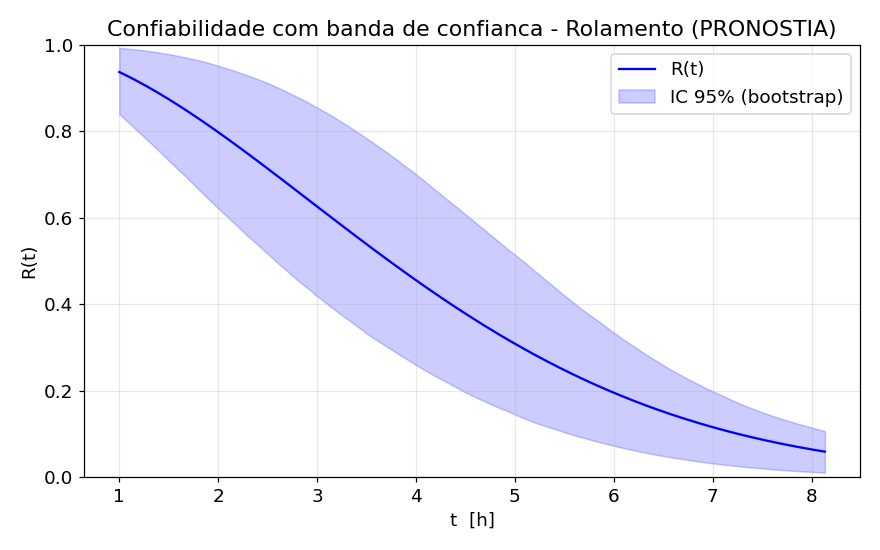
\includegraphics[width=\linewidth]{p5_R_banda_pronostia_all.png}\\[2pt]
            \footnotesize $R(t)$ (confiabilidade) com banda \textit{bootstrap}. Eixo $x$: tempo (h); eixo $y$: prob.\ de sobreviver.
        \end{center}
        \column{0.5\textwidth}
        \begin{center}
            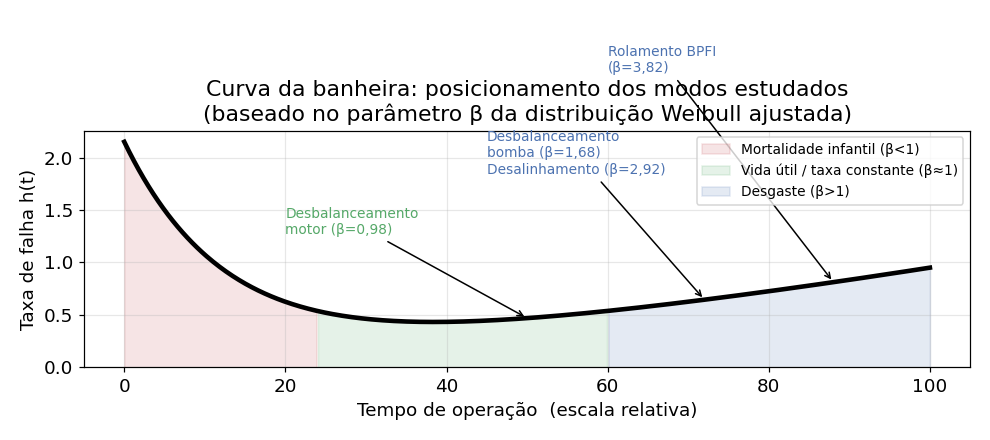
\includegraphics[width=0.86\linewidth]{curva_banheira.png}
        \end{center}
        \begin{block}{Desgaste, não mortalidade infantil}
            \tiny A região da banheira depende da \textbf{forma} ($\beta$), \textbf{não} da velocidade da falha. $\beta{=}1{,}80$ (IC $[1{,}39;\,2{,}88]$, todo $>1$) $\Rightarrow$ taxa \textbf{crescente} $=$ desgaste/fadiga. A aceleração só \textbf{encurta a vida} ($\eta$); não vira mortalidade infantil (que exigiria $\beta{<}1$). O MTTR de 24\,h afeta só a \textbf{disponibilidade}, não a banheira.
        \end{block}
    \end{columns}
\end{frame}

% =====================================================================
\section{Modelo de Sistema}
% =====================================================================

% Slide: monte carlo do sistema
\begin{frame}{Passo 6: modelo do sistema (Monte Carlo)}
    \scriptsize
    Neste passo modelamos um sistema imaginário composto por \textbf{dois rolamentos em série} (a falha de um derruba o conjunto). Simulam-se 3 arquiteturas para comparar como redundâncias afetam esse sistema:
    \vspace{0.15cm}
    \begin{itemize}
        \item \textbf{Série:} apenas um conjunto. \hfill $t = \min(t_1, t_2)$
        \item \textbf{Paralelo:} dois conjuntos ativos. \hfill $t = \max(t_A, t_B)$
        \item \textbf{Standby (reserva fria):} reserva entra após a 1ª falha. \hfill $t = t_A + t_B$
    \end{itemize}
    \vspace{0.15cm}
    \begin{block}{Disponibilidade verificada analiticamente}
        Série: $A=A_1 A_2$;\quad Paralelo: $1-(1-A)^2$;\\
        Standby: $\dfrac{\mu^2+\mu\lambda}{\mu^2+\mu\lambda+\lambda^2}$ (onde $\lambda$ é a taxa de falha e $\mu$ é a taxa de reparo).
    \end{block}
    \vspace{0.1cm}
    \begin{block}{Como se obtém $R(2\,\text{h})$ (confiabilidade de missão)}
        \scriptsize Para cada arquitetura, simulam-se $10^5$ vidas do sistema: sorteia-se a vida de cada unidade pela Weibull ajustada e combina-se pela fórmula de $t$ acima, obtendo o tempo de falha do sistema $T_{\text{sist}}$ de cada simulação. $R(2\,\text{h})$ é a \textbf{fração} das $10^5$ simulações com $T_{\text{sist}} > 2\,\text{h}$ (ainda vivas em 2\,h). A missão de 2\,h $\approx$ metade do MTTF de uma unidade.
    \end{block}
\end{frame}

% Slide: resultados do sistema
\begin{frame}{Passo 6: resultados do sistema}
    \begin{columns}
        \column{0.48\textwidth}
        \scriptsize
        \begin{tabular}{lcc}
            \toprule
            \textbf{Config.} & \textbf{Disp.} & $R(2\,\text{h})$ \\
            \midrule
            Série    & 0,02100 & 0,636 \\
            Paralelo & 0,04157 & 0,869 \\
            Standby  & 0,11385 & \textbf{0,965} \\
            \bottomrule
        \end{tabular}
        \vspace{0.2cm}
        \begin{itemize}
            \item MTTF do conjunto em série (dois rolamentos) $= \mathbf{3}$\,h.
            \item Analisou-se $R(2\,\text{h})$ (sobrevivência até a metade do MTTF original) como \textbf{missão} ilustrativa. Standby aumenta enormemente as chances de cumprir essa missão (96,5\%).
            \item A Disponibilidade do Standby é muito maior, mas o paralelo oferece resposta imediata caso um falhe.
        \end{itemize}
        \column{0.52\textwidth}
        \begin{center}
            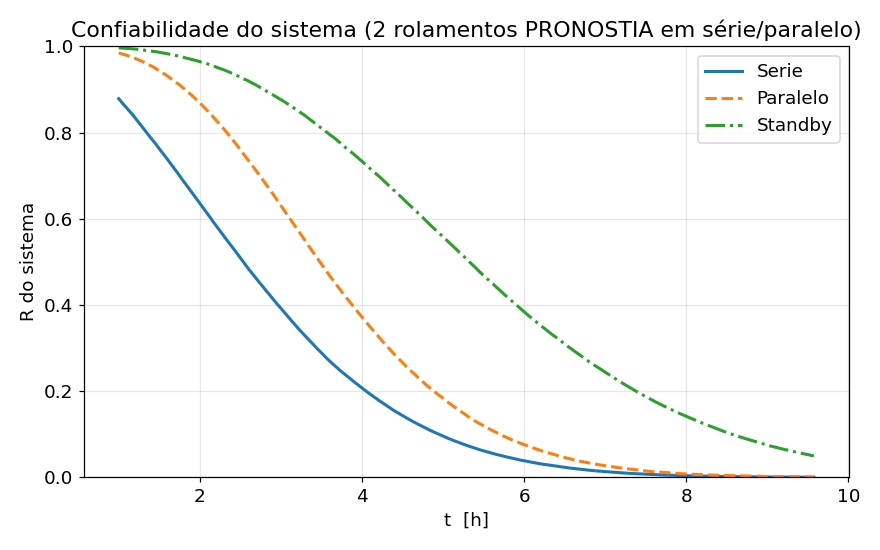
\includegraphics[width=\linewidth]{p6_sistema_R.png}
        \end{center}
    \end{columns}
\end{frame}

% =====================================================================
\section{Referências}
% =====================================================================
\begin{frame}{Referências}
    \footnotesize
    \begin{thebibliography}{9}
        \setbeamertemplate{bibliography item}[text]
        \bibitem{nectoux} P. Nectoux \textit{et al.}, ``PRONOSTIA: An experimental platform for bearings accelerated degradation tests,'' \textit{IEEE Int. Conf. on PHM}, 2012.
        \bibitem{oconnor} P. O'Connor, A. Kleyner, \textit{Practical Reliability Engineering}, 5ª ed., Wiley, 2012.
        \bibitem{meeker} W. Meeker, L. Escobar, \textit{Statistical Methods for Reliability Data}, Wiley, 1998.
        \bibitem{colosimo} E. Colosimo, S. Giolo, \textit{Análise de Sobrevivência Aplicada}, Blucher, 2006.
        \bibitem{robert} C. Robert, G. Casella, \textit{Introducing Monte Carlo Methods with R}, Springer, 2010.
        \bibitem{zio} E. Zio, \textit{The Monte Carlo Simulation Method for System Reliability and Risk Analysis}, Springer, 2013.
        \bibitem{reid} M. Reid, \textit{reliability} --- Python library for reliability engineering, Zenodo, 2024.
        \bibitem{bessani} M. Bessani, Notas de aula --- EEE017 Confiabilidade de Sistemas, UFMG, 2026.
    \end{thebibliography}
\end{frame}

\end{document}
